\begin{surferPage}[Cayley-Cubica]{La Cubica di Cayley}
   Questa superficie cubica (superficie di grado $3$) compare anche nella galleria sulle superfici semplici. In tutto, essa ha quattro singolarit\`a a cono doppio. Il nome di questa superficie \`e in onore di Arthur Cayley, che studi\`o molto le cubiche nel XIX secolo.
   
  Fu tuttavia Ludwig Schl\"{a}fli il primo a classificare in modo sistematico queste superfici nel 1863 a seconda delle loro possibili singolarit\`a. 
  Per esempio, nel suo articolo \`e spiegato perch\'e non vi possono essere pi\`u di $4$ punti singolari su una superficie cubica. Pertanto $\mu(3)=4$. 
    
    Intorno al 1900, Felix Klein studi\`o le possibili forme delle superfici cubiche reali; la sua idea fu di rispondere a questa domanda partendo dalla Cubica di Cayley tramite piccole deformazioni. Espandendo le singolarit\`a a cono doppio, staccando o unendo parti, Klein fu in grado di trovare tutte le possibili forme; eccone alcune: 
    \vspace{0.3cm}
     \begin{center}
      \vspace{-0.2cm}
      \begin{tabular}{@{}c@{\ }c@{\ }c@{\ }c@{}}
        \begin{tabular}{@{}c@{}}
          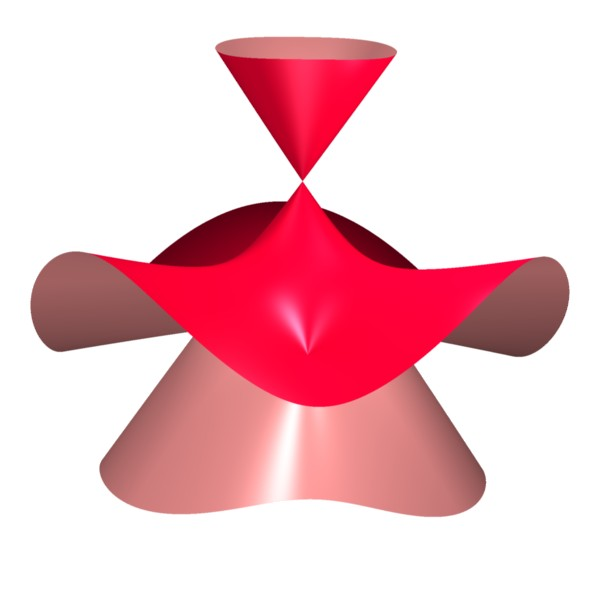
\includegraphics[width=1.35cm]{./../../common/images/cayley_cubic_0}
        \end{tabular}
        &
        \begin{tabular}{@{}c@{}}
          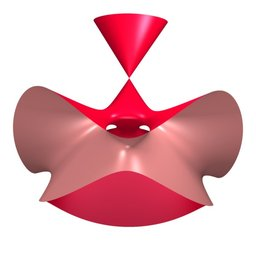
\includegraphics[width=1.35cm]{./../../common/images/cayley_cubic_1}
        \end{tabular}
        &
        \begin{tabular}{@{}c@{}}
          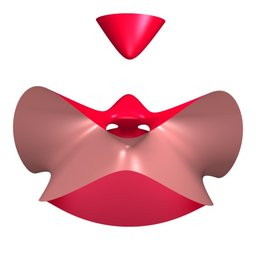
\includegraphics[width=1.35cm]{./../../common/images/cayley_cubic_2}
        \end{tabular}
        &
        \begin{tabular}{@{}c@{}}
          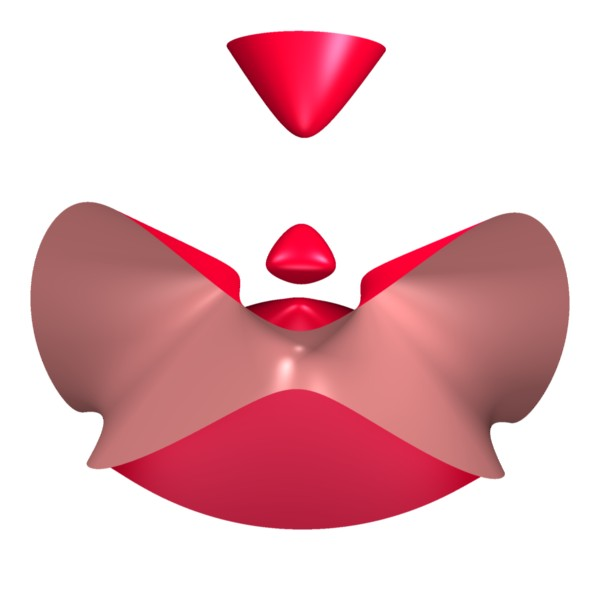
\includegraphics[width=1.35cm]{./../../common/images/cayley_cubic_3}
        \end{tabular}
      \end{tabular}
    \end{center}
\end{surferPage}
